\section*{Brainstorm}
\begin{figure}[H]
	\centering
	\begin{tikzpicture}
	\path[mindmap,
	every node/.style=concept,
	concept color=black,
	scale=0.5,
	text=white,
	text width=2cm,
	grow cyclic,
	level 1/.append style={level distance=8.5cm,sibling angle=70},
	level 2/.append style={level distance=6cm,sibling angle=45}]
	node[concept] {Simple sketch to virtual world}
	[clockwise from=-20]
	child[concept color=green!50!black] {
		node[concept] {Building}
		[clockwise from=-20]
		child { node[concept] {Over construction} }
		child { node[concept] {Overuse of materials} }
	}  
	child[concept color=black!20!blue] {
		node[concept] {Architecture}
		[clockwise from=-67]
		child { node[concept] {Sketching} }
		child { node[concept] {3D modeling} }
	}
	child[concept color=orange] { node[concept] {Presentation} [clockwise from=-90]
		child { node[concept] {Teachers}}
		child { node[concept] {Students}}
	};
	\end{tikzpicture}
	\captionof{figure}{The outcome of the intitial brainstorm}
	\label{fig:brainstorm}
\end{figure}
\section*{Interview Questions for plant center customers}\label{sec:interviewQuestionsCustomer}
% when and where
% what does location and time mean for the data
List of questions for target group
\begin{itemize}
	\item[-] Have you ever used a garden designer?
	\item[-] What was your experience?
	\item[-] What are you planning to buy?
	\item[-] What are you plan/thoughts for when you buy a new plant?
	\item[-] What do you consider when you buy a new item for your garden?
	\item[-] How often do you make major changes to your garden?
	\item[-] For which reasons did you decide to purchase this item?
	\item[-] What was the latest item you bought that you were not satisfied with?
	\item[-] Do you have a garden?
	\item[-] How did you start the design process?
	\item[-] What tools did you use, if any?
	\item[-] When did you make changes to your garden?
	\item[-] What big changes would you like to make?
	\item[-] Are you retired?
	\item[-] If you had all the time in the world, what would you change about your garden?
	\item[-] Do you enter the garden center with a budget in mind?
	\item[-] Why are you here? \\
\end{itemize}

\paragraph*{Demographic information}
\begin{itemize}
	\item[-] Sex
	\item[-] Age
	\item[-] Job
	\item[-] Marital Status
	\item[-] Level of education
\end{itemize}


\section*{Interview Questions for experts}\label{sec:interviewQuestionsExperts}
This is a rough outline of the questions we asked the experts. The translated version (and the original Danish version) of each question is listed below. Since the interview was semi-structured all questions were not necessarily used or not used in exactly in the form written here.\\

Personal questions:
\begin{itemize}
	\item[-] How did you end up in this business? (Hvordan er du endt i den her branche?)
	\item[-] What is your role in the company? (Hvad er din rolle i virksomheden?)
	\item[-] What does your workday consist of? (Hvad består din arbejdsdag af?)\\
\end{itemize}

Design questions:
\begin{itemize}
	\item[-] How large of a garden area do you usually work with? (Hvor stort haveareal arbejder I med normalt?)
	\item[-] What plants, trees or other elements are trending at the moment? (Hvilke planter, træer eller andre have elementer, hitter lige nu?)
	\item[-] What is a popular garden style? (Hvad er en populær have stil?)
	\item[-] Do many people want to have a lake or a fishpond built in the garden? (Er der mange der får lavet søer eller fiskedamme i haven?)
	\item[-] What do you need to be specifically aware of when designing garden in Denmark? (Hvad skal man være specielt opmærksom på når man designer haver i Danmark?)
	\item[-] How do you show/demonstrate a final design for the clients? (Hvordan viser/demonstrere du færdige designs til kunderne?)\\
\end{itemize}

Target group questions:
\begin{itemize}
	\item[-] What kind of people do usually contact you? (Hvilke mennesker henvender sig mest til jer/dig?)
	\item[-] What is the most usual demography? (Hvad er den mest almindelige demografi?)
	\item[-] Is it usually private clients or is it municipal clients (Er det primært privatpersoner eller er det kommuner, der er jeres kunder?)
	\item[-] Do people need designing for the whole garden or just parts of their garden? (Skal folk have lavet hele haven eller er det kun dele af haven?)
	\item[-] Who makes the 3D visualization of the garden? Is it something you create internally in the company, or does it come from outside cooperators? 
	\item[-] How much influence do the clients have in the process? (Hvor meget indflydelse har kunderne i processen?)\\
\end{itemize}

Technology questions:
\begin{itemize}
	\item[-] Do you offer 3D visualization of the gardens? (Tilbyder du/i 3D visualisering af haverne?)
	\item[-] Who is doing the 3D visualization of the garden? Are you doing it internally in the company or does it come from outside? (Hvem laver 3D visualiseringen af haven? Er det noget i laver internt i virksomheden, eller kommer det udefra?)
	\item[-] Why did you choose to offer this? (Hvorfor valgte i at tilbyde dette?)
	\item[-] For how long have you been offering this? (Hvor lang tid har i tilbudt dette?)
	\item[-] Do people take the offer on 3D visualization of their garden? (Benytter folk sig af tilbuddet om 3D visualisering af haven?)
	\item[-] Can you see the development over time? (Kan man se udviklingen over tid?)
	\item[-] Does this mean that the growth can be followed year by year, or is it about the seasons? (Betyder det at væksten kan følges år for år, eller handler det om årstider?)
	\item[-] Is it something people make use of?\\
\end{itemize}

Project specific questions:
\begin{itemize}
	\item[-] How do you think a Virtual Reality experience in the 3D environment would be received? (Hvordan tror du at en VR oplevelse i 3D miljøet, ville blive modtaget?)
	\item[-] Is this a product that would be interesting for you in your process and how do you see this working? (Er det et produkt, der ville være interessant for jer, i jeres process, og hvordan forestiller du dig at det ville fungere?)\\
\end{itemize}

SOTA questions:
\begin{itemize}
	\item[-] Have you heard of this type of product before or something similar? (Har du hørt om denne type produkt før eller noget lignende?)
\end{itemize}

\section*{Interview transcriptions}\label{interviewTranscriptions}
Due to the large number of pages the complete transcriptions have not been included in this report. We refer you instead to the digital appendices. This section includes the Danish translations of the quotes used in this report:\\
\begin{comment}
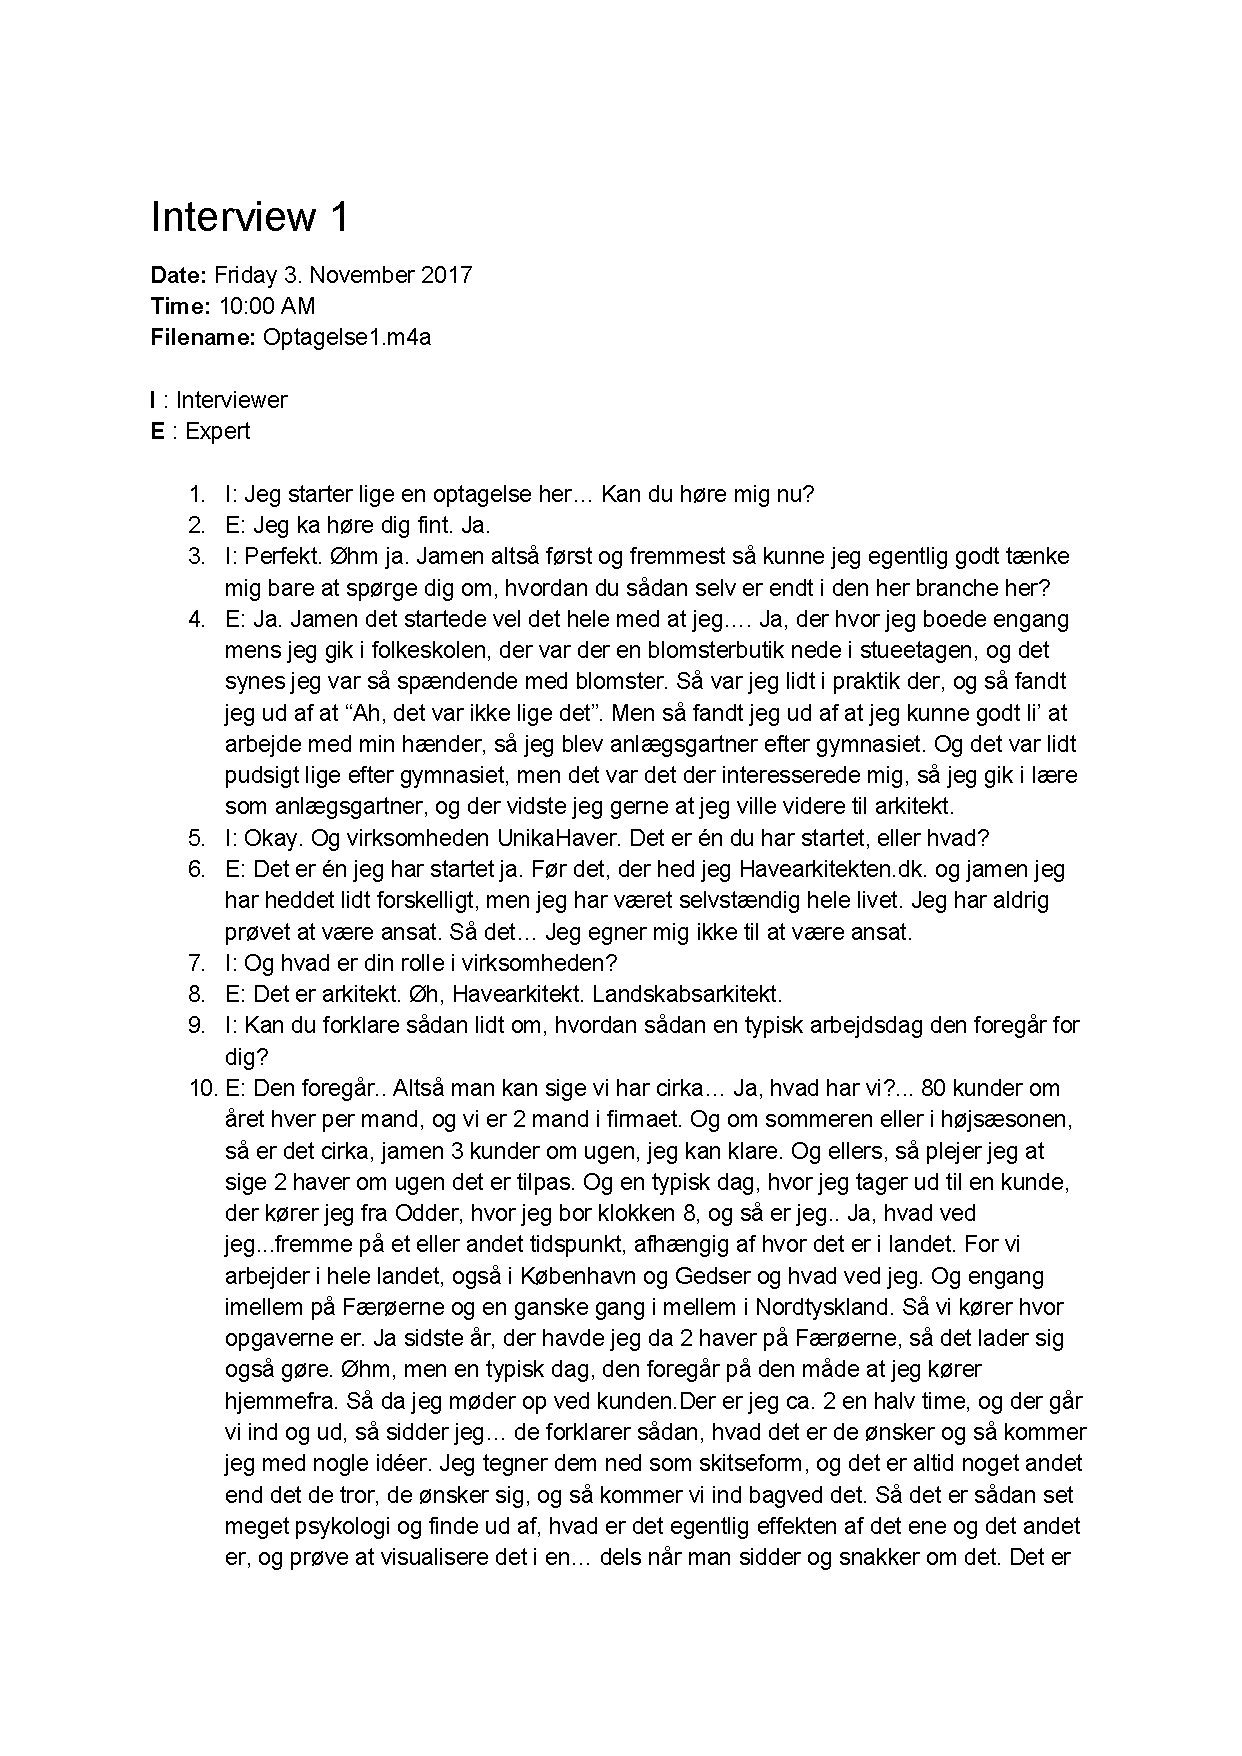
\includepdf[pages=-]{figure/Appendices/transcribedInterview1.pdf}
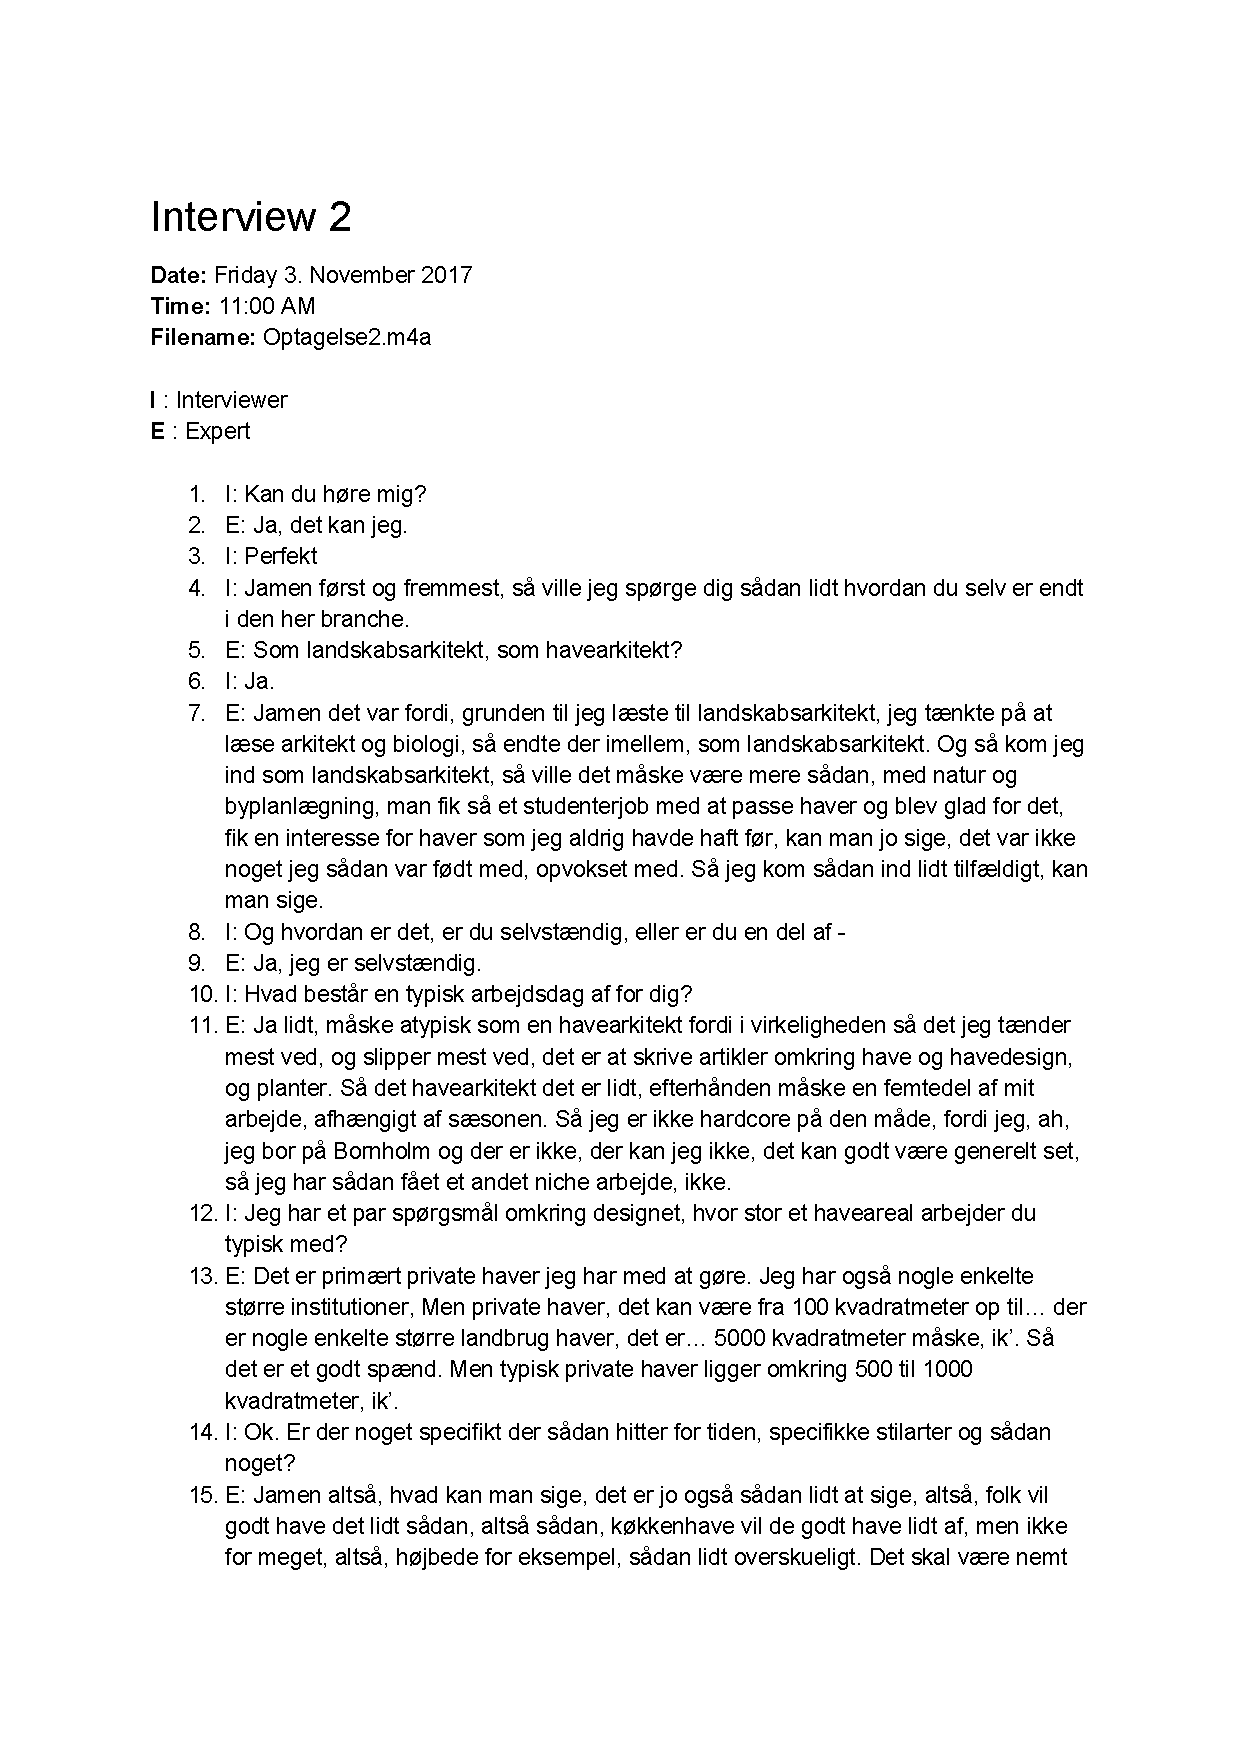
\includepdf[pages=-]{figure/Appendices/transcribedInterview2.pdf}
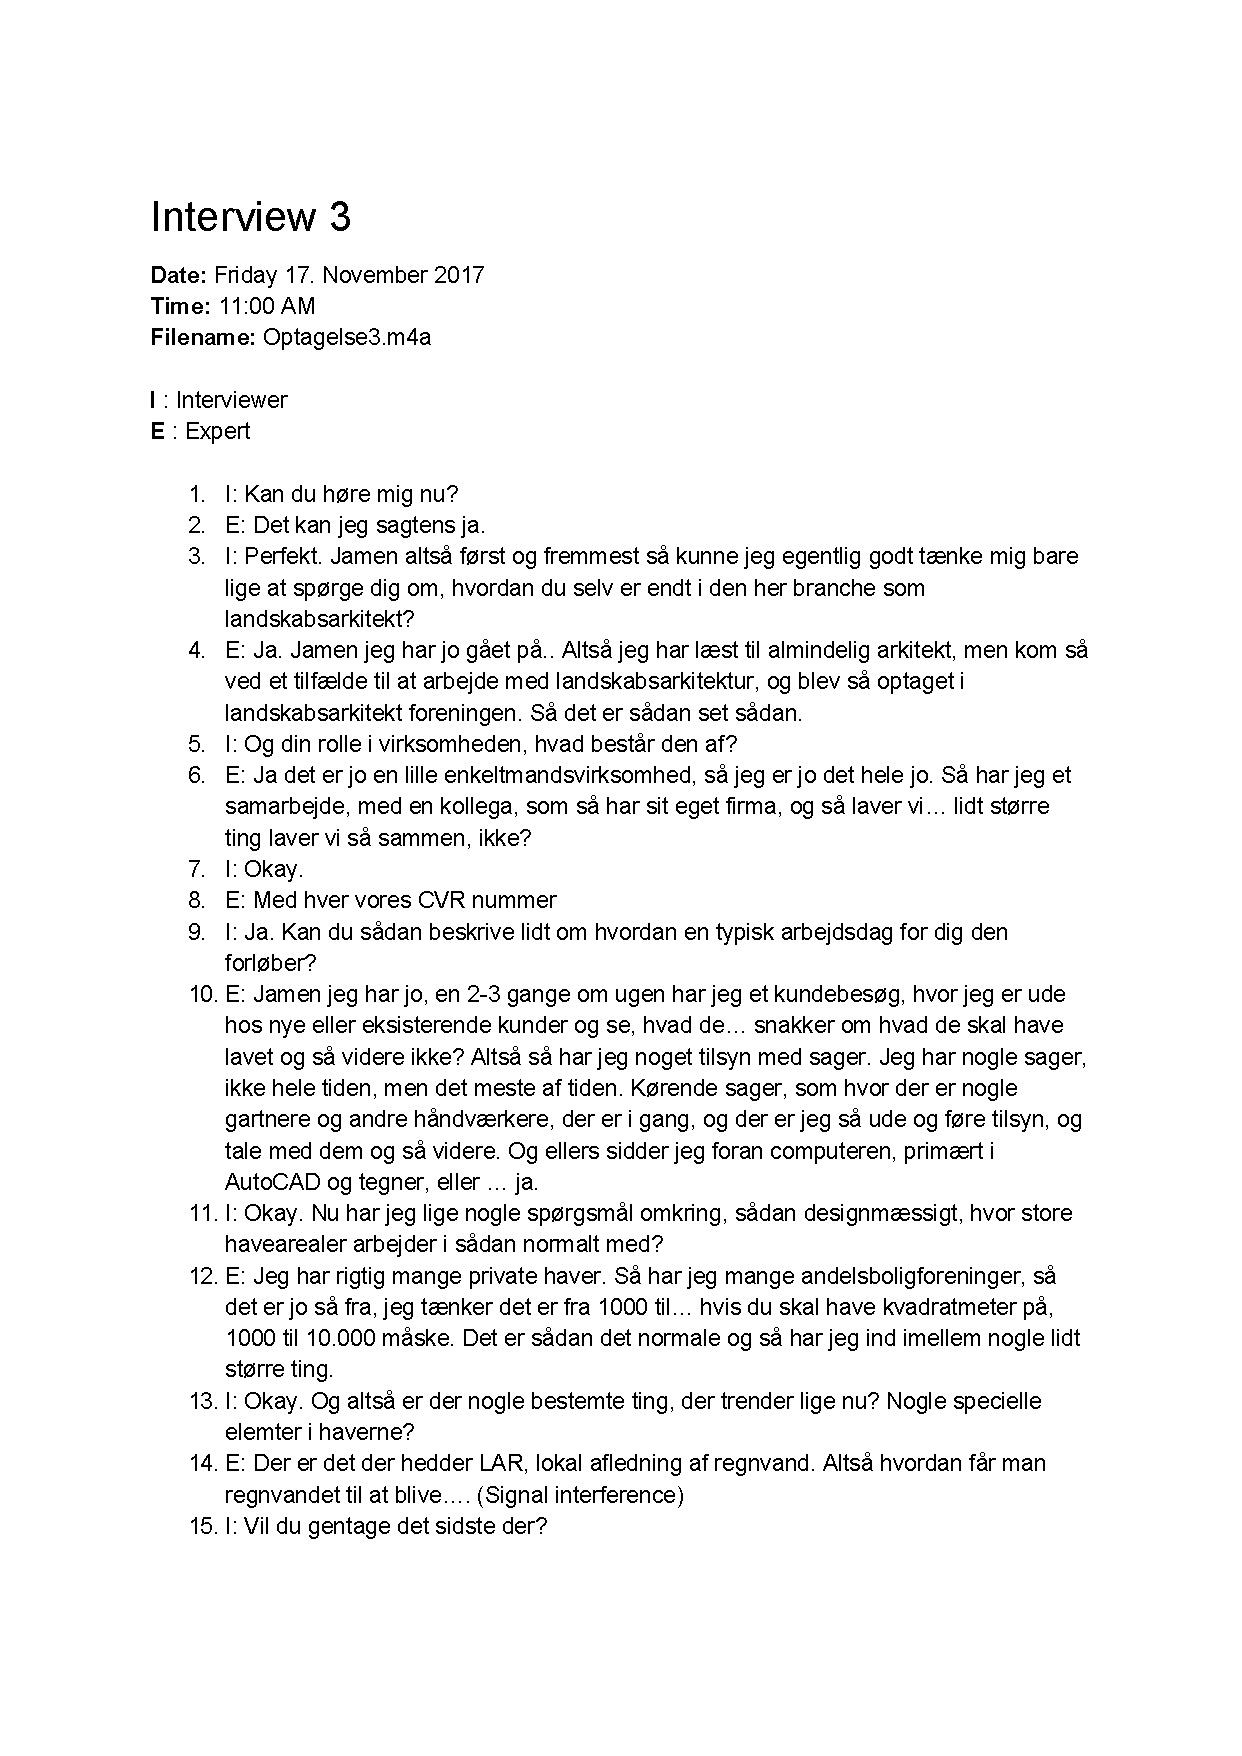
\includepdf[pages=-]{figure/Appendices/transcribedInterview3.pdf}
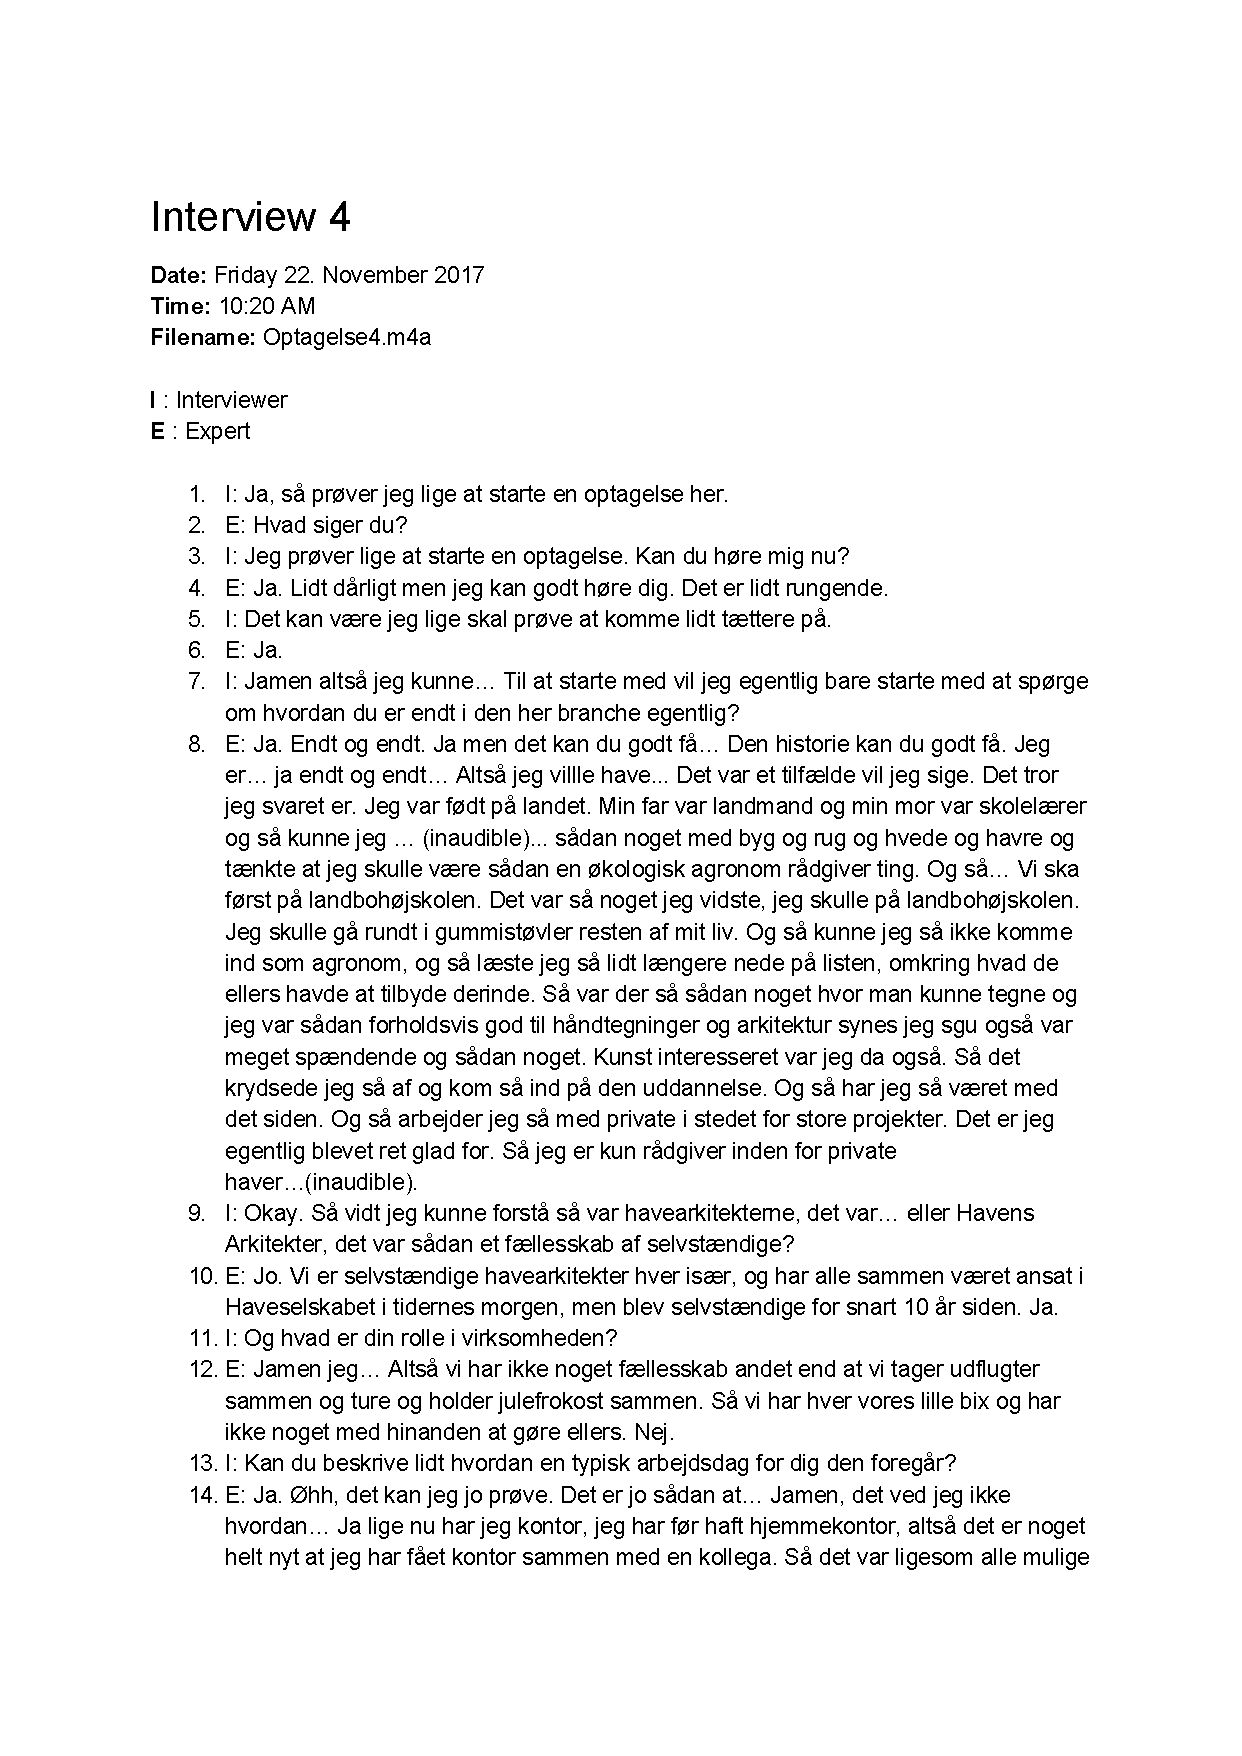
\includepdf[pages=-]{figure/Appendices/transcribedInterview4.pdf}
\end{comment}


\paragraph*{Process:}
\begin{quote}
	\textit{Så da jeg møder op ved kunden.Der er jeg ca. 2 en halv time, og der går vi ind og ud, så sidder jeg… de forklarer sådan, hvad det er de ønsker og så kommer jeg med nogle idéer}\label{quote:expertProcess1Danish}.\\
\end{quote}

\begin{quote}
	\textit{Det er sgu ikke vores mening, der skal frem. Vi fortæller bare, hvad man kan gøre og ikke kan gøre og så skal de egentlig bare hjælpe os med at vælge fra og vælge til}\label{quote:expertProcess2Danish}.\\
\end{quote}

\begin{quote}
	\textit{Ja, jeg prøver jo virkelig at få dem så meget med jeg kan, fordi jeg ved at, at, jeg er blevet mere bevidst om hvor meget jeg kan påvirke dem. [...] Men nu lytter jeg synes jeg mere, til hvad de egentlig har brug for. }\label{quote:expertProcess3Danish}\\
\end{quote}

\paragraph*{Clients:}
\begin{quote}
	\textit{Altså hvis det er private kunder, så er de fra midt 40’erne tit. Ja det ved jeg ikke. 40’erne 50’erne, og der er også nogle ældre}\label{quote:expertClients1Danish}.\\
\end{quote}

\begin{quote}
	\textit{Jeg synes jeg oplever meget med folk, der har købt nyt hus med to børn. [...] Ej, de er i 30’erne ikke? 30,32,35 og så op efter ikke? Det er mellem 35 og 55-60.}\label{quote:expertClients2Danish}.\\
\end{quote}

\begin{quote}
	\textit{Det er faktisk nede i 20’erne. [...] Ja, altså der er jo sindssygt mange midt i tyverne, der bygger hus.}\label{quote:expertClients3Danish}.\\
\end{quote}

\begin{quote}
	\textit{det er i hvert fald 40+, ik’? Altså på Bornholm kan det godt være unge}\label{quote:expertClients4Danish}.\\
\end{quote}

\paragraph*{Design:}
\begin{quote}
	\textit{altså at man går ind på græsplænen og ikke ud på græsplænen. Altså hvis vi kan sige at vi går ind hele tiden, jamen så er vi i mål. Så det er sådan nogle små ting vi opererer med, når vi tænker rum og former og figurer. Det er hele tiden, at vi skal psykologisk mærke at vi er inde her. “Ahh inde i varmen” hele tiden.}\label{quote:expertDesign1Danish}\\
\end{quote}

\begin{quote}
	\textit{Det er der faktisk meget langt imellem at nogen ønsker sig rindende vand. Man kan sige, engang imellem så er der nogen der ønsker sig spejlbassiner.}\label{quote:expertDesign2Danish}\\
\end{quote}

\begin{quote}
	\textit{Ja, altså du skal jo vælge planter som egner sig til dansk klima.}\label{quote:expertDesign3Danish}\\
\end{quote}

\begin{quote}
	\textit{Men trenden, er at det skal være vedligeholdesesfrit. Det er i hvert fald et af toppunkterne. Det skal være nemt at holde. Så skal det se pisse godt ud, og det behøver ikke at koste en milion.}\label{quote:expertDesign4Danish}\\
\end{quote}

\paragraph*{Technologies:}
\begin{quote}
	\textit{Altså for os der er Google Sketchup så absolut det nemmeste at arbejde i. Altså vi har begge to også kørt med AutoCAD førhen, og det er simpelthen så tungt at danse med}\label{quote:expertTech1Danish}.\\
\end{quote}

\begin{quote}
	\textit{så laver jeg en SketchUp tegning, som jeg arbejder videre med i PhotoShop eller på en anden måde. Og det er faktisk noget, der fungerer fint til min type opgaver}\label{quote:expertTech2Danish}.\\
\end{quote}

\begin{quote}
	\textit{Primært er det fordi at hvis jeg bruger 2-3 timer på en have, så kan jeg ikke bruge 2 timer på at lave noget 3D, fordi så bliver det en dobbelt dyr haveplan}\label{quote:expertTech3Danish}.\\
\end{quote}

\begin{quote}
	\textit{Og så fordi, hvis jeg skulle have det med hjem, så skulle jeg jo sidde og arbejde med det every day. Og det kommer til at blive en for dyr en process i forhold til hvad jeg sælger til kunden
	}\label{quote:expertTech4Danish}.\\
\end{quote}

\paragraph*{Visualising space}

\begin{quote}
	\textit{Pludselig, så kan dem, der har svært ved at forestille sig noget rummeligt, fornemme hvad er det vi er på vej hen til, fordi det havde de ikke en chance for før. Altså der er virkelig mange, der slet ikke har nogen rummelig forståelse. Og tegningen skal ligge fuldstændig sådan som huset nu ligger på bordet, for ellers så bliver de fuldstændig rundtossede}\label{quote:expertRoom1Danish}.\\
\end{quote}

\begin{quote}
	\textit{Det er mest, hvis jeg synes at jeg skal illustrerer noget, som er svært for dem at forstå.}\label{quote:expertRoom2Danish}\\
\end{quote}

\begin{quote}
	\textit{jeg har den der dialog, så folk meget bedre kan fornemme rummeligheden, fordi jeg forklarer højder og alt muligt.}\label{quote:expertRoom4Danish}\\
\end{quote}

\begin{quote}
	\textit{Altså fordi, de får det jo en lille smule, når jeg sidder og skitserer og tegner på stedet og det bliver farvelagt, så pludselig, så kan jeg mærke, så rammer jeg simpelthen også hustruen ikke? Fordi der er sgu tit dem der ikke… kvinderne, der ikke kan se det her 3D ting, så siger de: “Gud nu forstår jeg det bare”.}\label{quote:expertRoom3Danish}\\
\end{quote}

\begin{quote}
	\textit{Og jeg kan vise det samme ved at stå ude i haven. [...] Men det er et spørgsmål for mig om folk vil give de penge det nu koster at visualisere, altså man kan også blive forført af den visualisering, man kan gå rundt og man kan se og det er smart, ik’, men hvad er det egentlig. Men så skulle man have to forskellige visualiseringer, så man kan se, det er den ene løsning og det er den anden løsning og hvad er så bedst, for ellers er det ligesom, så er det bare en smart feature som ser godt ud og virker lidt tjekket, men du er ikke inde og reelt sådan måske, du kan, det jeg tænker er lidt, du kan falde på halen over teknikken, og sige nej det er fedt, uden at egentlig oplever, det ved jeg ikke om du oplever haven eller om du bare bliver fascineret af det, af teknikken der ligger omkring at lave en 3D, ik’.}\label{quote:expertRoom5Danish}\\
\end{quote}



\paragraph*{Resources:}
\begin{quote}
	\textit{Hvis vi laver 80 på et år i alt, jamen så er det vel 15, der får 3D. 15 ud af 80.}\label{quote:expertRessources1Danish}.\\
\end{quote}

\begin{quote}
	\textit{Altså faktisk, så ville jeg tro at de fleste ville gøre det, hvis det ikke var så meget dyrere}\label{quote:expertRessources2Danish}.\\
\end{quote}

\begin{quote}
	\textit{Altså det som jo er grunden til at man ikke bruger det mere, det er fordi det tager jo… det tager mange dage at lave sådan en god tegning. Og 700 kroner i timen gange mange dage, det er de færreste, der vil betale det}\label{quote:expertRessources3Danish}.\\
\end{quote}

\begin{quote}
	\textit{hvis det er grænseoverskridende for mig at sige at sådan en tegning skal koste 7000, ikke? Det synes jeg, må men det er egentlig forholdsvis mange penge, ikke?}\label{quote:expertRessources4Danish}.\\
\end{quote}

\paragraph*{Ideas:}
\begin{quote}
	\textit{Fordi jeg har jo sådan set lavet tegningen. Men kunne jeg få lavet en 3D version, som kunne gøres så hurtigt, at jeg egentlig bare lavede en rentegning af skitsen i 3D, så synes jeg måske, at det ville være en opgradering, men så har det jo ikke nogen planteliste, så er det bare tegningen i 3D. Men det er det prisleje, jeg tænker kunne, det kunne være interessant for mig at arbejde med det i, ikke?}\label{quote:expertIdeas1DanishDanish}\\
\end{quote}

\begin{quote}
	\textit{Og det ville være rigtig fint, hvis man kunne lave nogle rummelige fremstillinger nemmere, fordi så ville man kunne bruge det langt langt mere. Altså jeg ville jo synes det var fantastisk, hvis jeg kunne sende noget med til mine almindelige kunder, som jeg ikke har brugt 3 dage på at lave}\label{quote:expertIdeas2Danish}.\\
\end{quote}

\begin{quote}
	\textit{Altså helt ideelt, så ville det være at, når jeg nu i min process med kunden der, på de to og en halv time har siddet og skitserer frem til et eller andet, og så ville det være helt super fedt… Altså et eller andet sted så kunne det godt være at det bare var 3D, der rejste sig op simpelthen ud af papiret}\label{quote:expertIdeas3Danish}.\\
\end{quote}

\begin{quote}
	\textit{Og hvis man kunne tage en brille på og så tegne ud i luften, altså så var det jo interessant}\label{quote:expertIdeas4Danish}.\\
\end{quote}



\section*{Marker auto-generating program}
The code shown in Listing \ref{listing:generatorCode} is the Processing code used to generate markers given just an integer array as input. The program was developed using Processing.

\begin{listing}[H]
	\caption{Code for the marker auto-generating program}
	\label{listing:generatorCode}
	\begin{minted}[frame=lines,
		framesep=2mm,baselinestretch=1.1,fontsize=\footnotesize,linenos]{java}
int[] markers = {1, 2, 4, 8,16,32,64,128,100,3,9};
int spacing = 800;
PImage circle;
PImage values[] = new PImage[8];
void setup() {
	circle = loadImage("circle.png");
	for (int i = 0; i<values.length; i++) {
		values[i] = loadImage(""+int(pow(2, i))+".png");
	}
	size(3508, 4961);
	surface.setVisible(false);
	background(255);
	//4x6 markers on a3 paper
	int x = 0;
	int y = 0;
	int counter=0;
	for (int i = 0; i<markers.length; i++) {
		drawMarker(markers[i], x, y);
		x++;
		if (x>3) {
			x = 0;
			y++;
			if(y>4){
				save("result"+counter+".png");
				counter++;
				x=0;
				y=0;
				
			}
		}
	}
	save("result"+counter+".png");
	exit();
}

void drawMarker(int num, int xpos, int ypos) {
	int x = spacing/2+xpos*spacing;
	int y = spacing/2+ypos*spacing;
	String str = binary(num, 8).toString();
	int s = int(circle.width*1.5);
	image(circle, x, y,s,s);
	
	for (int i = 0; i<8; i++) {
		if (str.charAt(i)=='1') {
			tint(0,255);
			image(values[7-i], x, y,s,s);
			tint(255);
		}
	}
	
}
	\end{minted}
\end{listing}

\section{Usability test}

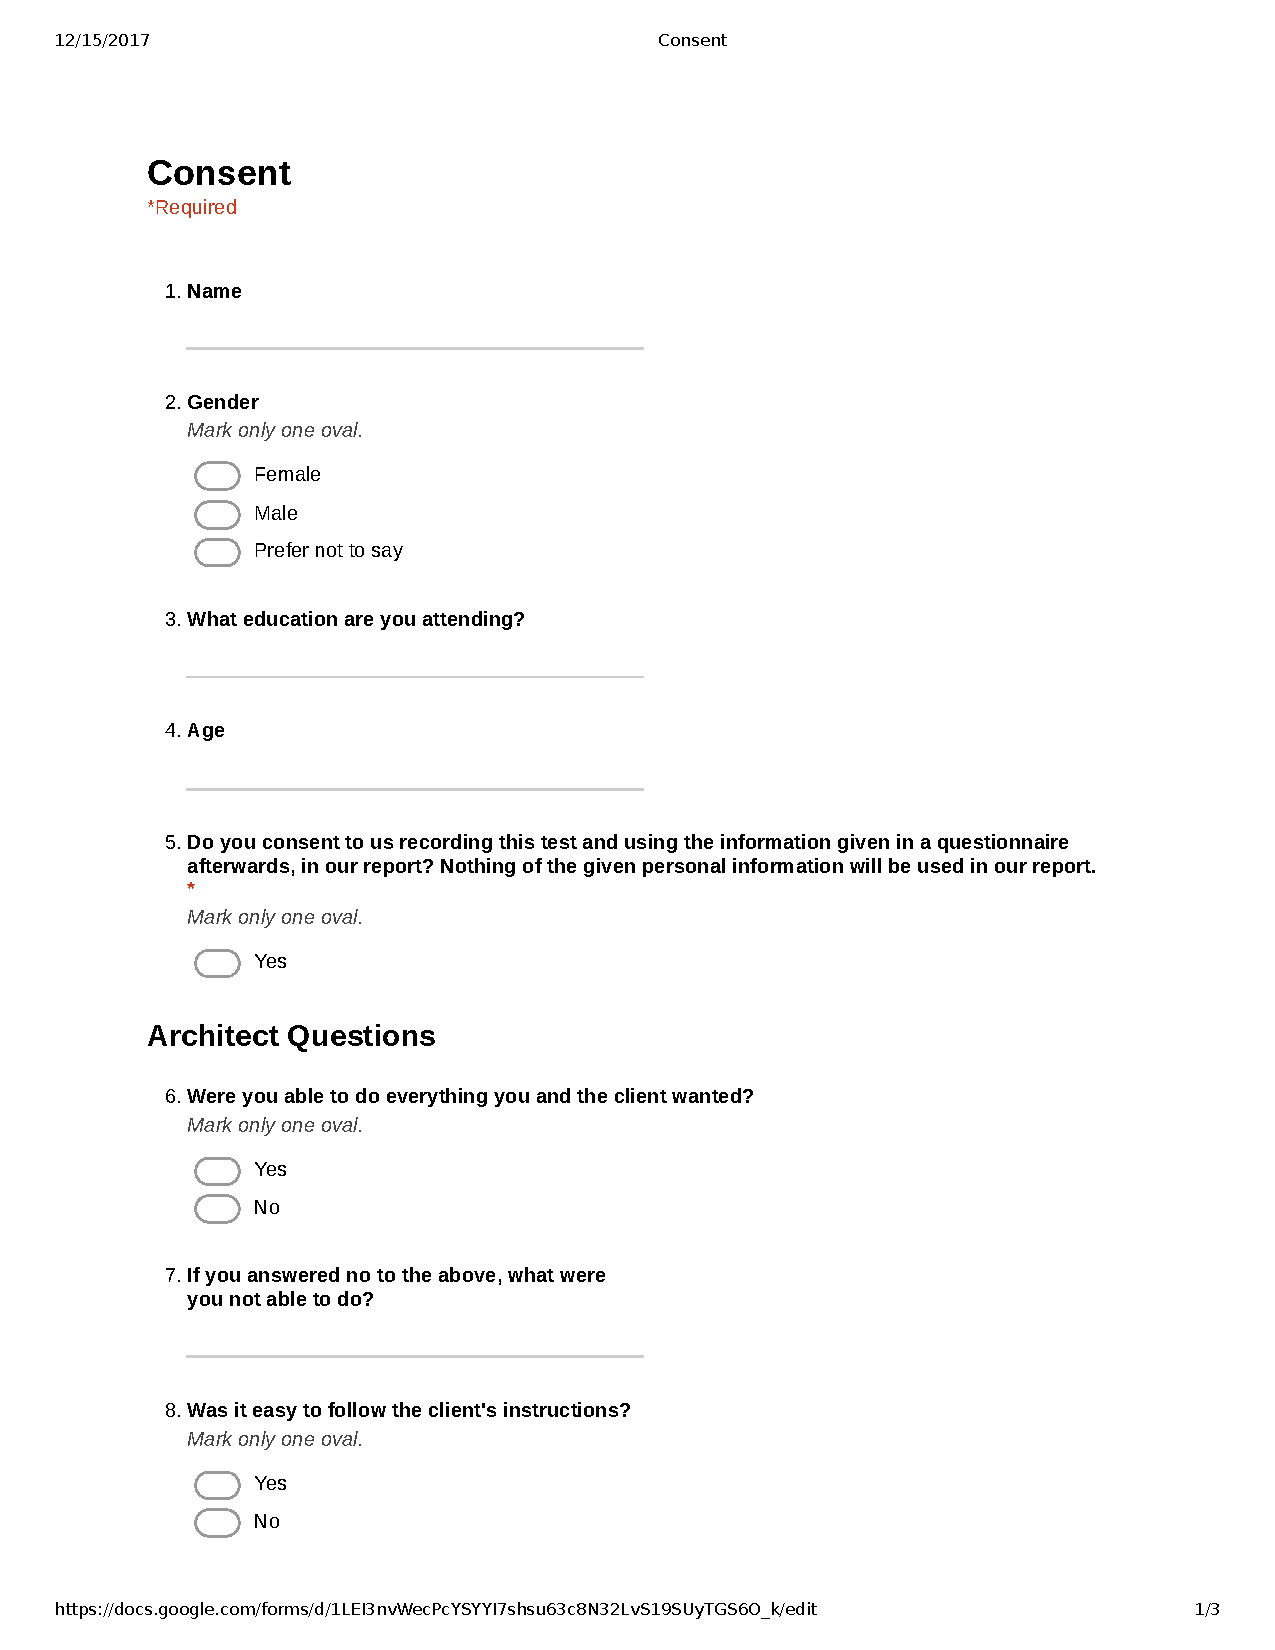
\includepdf[pages=-]{include/Appendices/architect.pdf}
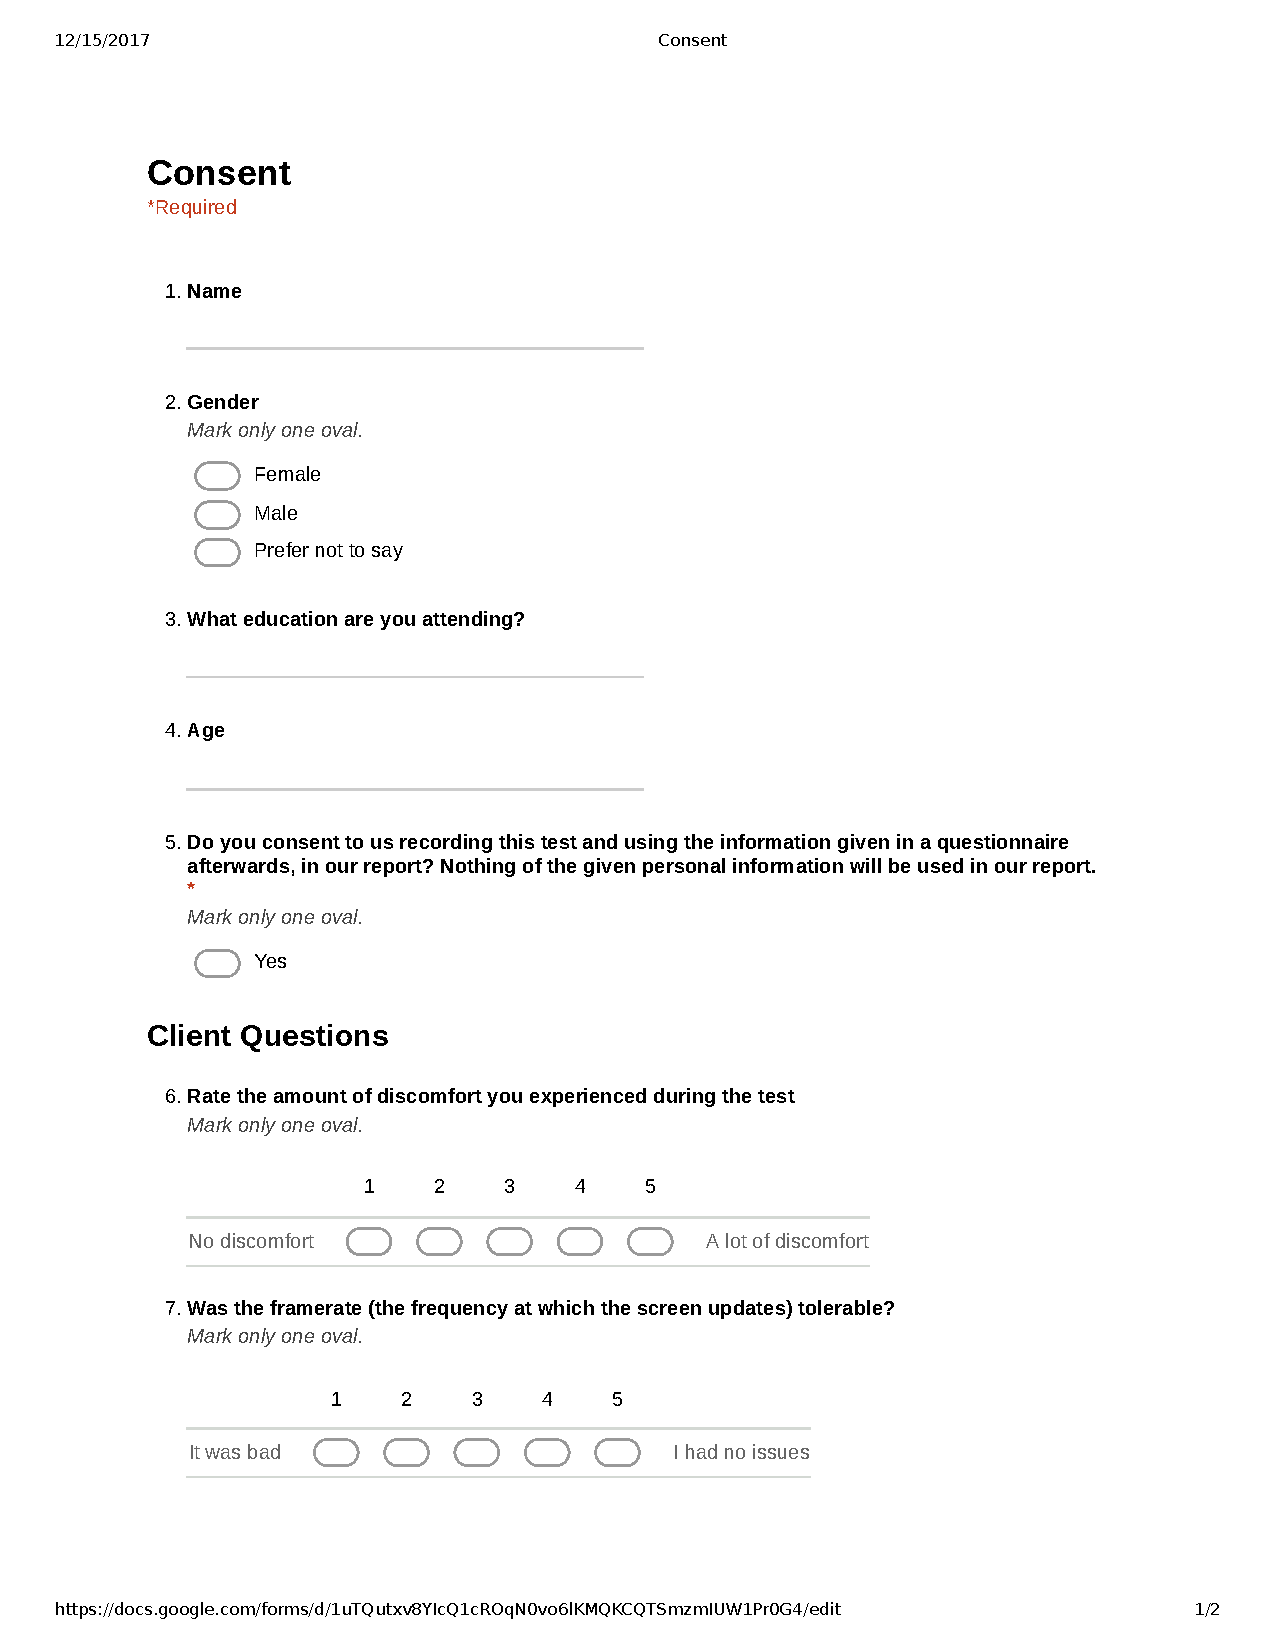
\includepdf[pages=-]{include/Appendices/client.pdf}

